\documentclass[]{article}
\usepackage{listings}
\usepackage{hyperref}
\usepackage{xcolor}
\usepackage{geometry}
\usepackage{csquotes}
\usepackage[]{setspace}
\usepackage[]{graphicx}
\usepackage[]{amsmath}
\usepackage[]{amsfonts}
\usepackage[]{hyperref}
\usepackage{caption}
\usepackage{subcaption}
\usepackage{graphicx}
\usepackage[
backend=biber,
style=authoryear-comp,
sorting=ynt]{biblatex}
\addbibresource{phdreflib.bib}

\geometry{margin=1in}
\setlength{\parskip}{6pt}
\setlength\parindent{0pt}
\setstretch{1}

%opening
\title{From Neural to Social Computation: Collective Intelligence in Networks of Complex Agents}
\author{Marie-Lou Laprise\footnote{Some of the ideas for this project were developed in collaboration with Kamesh Krishnamurthy (Princeton Physics \& PNI)}}

\begin{document}
	
	\maketitle
	
``Think how hard physics would be if particles could think" --Murray Gell-Mann

\section{Introduction: Seeking inspiration from neural computation to model social dynamics}
A variety of complex systems across scales, from colonies of ants to neurons in the brain, exhibit the capacity to map noisy inputs to useful outputs in a decentralized, emergent manner: they perform distributed computation.\footnote{ I loosely follow Crutchfield (\cite{crutchfieldCalculiEmergenceComputation1994}) by defining \textbf{computation} as a useful mapping from an input to an output; and \textbf{distributed} to mean that computation emerges from the time-varying state of a system of many interacting elements.} Social networks also do so; a prominent example being price discovery in financial markets. However, this remains a blind spot for both social science and theories of collective computation. Social scientists tend to study decision-making by looking at individual behaviors or aggregate outcomes. They rarely take a complex systems approach, and they have not thought of social networks in terms of computation. On the other hand, existing models and theories of collective computation do not provide satisfactory explanations for the social setting, where agents are complex and heterogeneous. In neuroscience or biophysics, models often feature homogeneous, memory-less agents. In control systems and opinion formation studies, many models rely on linear dynamics that cannot replicate phenomena like threshold effects or information saturation.

How do social networks of heterogeneous agents collect and exchange noisy information to collectively form opinions and make decisions? Can we extend models of neural computation to explore this setting?

Interacting adaptive agents face some collective challenges that resemble those of neurons in the brain or nodes in an artificial network: (i) implementing distributed computation robustly and flexibly, over a range of time scales, and (ii) building predictive models of their environment. Together, I call tackling those goals collective intelligence. If there exists common principles underlying collective intelligence across settings, then models of neural computation may help us understand social computation. Conversely, models of social computation between complex agents might in turn suggest new models for how groups of neurons or regions of the brain interact to create a richer dynamical repertoire.

For instance, Naomi Leonard and colleagues developed a model of multi-agent opinion formation that takes a form similar to a recurrent neural network (RNN) (\cite{bizyaevaNonlinearOpinionDynamics2022}, \cite{leonardFastFlexibleMultiAgent2024}) (the “BFL” model). I describe it in Section 2 below. The BFL model introduced nonlinearity to better model information saturation, in contrast to the linear averaging models that dominated the field of opinion dynamics. The BFL model exhibits the ability to break indecision and rapidly converge to a steady state of consensus (all agents agree) or disagreement (agreement within subgroups but not between them) in a way that, its authors argue, parallels the observed behavior of bees choosing a nesting site or voters choosing a candidate.

The BFL model offered an elegant solution to a long-standing problem in the field of opinion formation: how to craft a system that may generate stable disagreement as a function of inputs and initial conditions, rather than one that inevitably converges to consensus or avoids consensus only at the cost of a fixed, carefully hand-picked connectivity matrix (\cite{ravazziDynamicalSocialNetworks2021}, \cite{bernardoBoundedConfidenceOpinion2024}). This problem is sometimes called Abelson's diversity puzzle (\cite{abelsonMathematicalModelsDistribution1964}).

The BFL model, however, features simple, homogeneous agents, without memory or intelligence.  For this project, I take a first step to improve this aspect of the BFL model by adding a unit-specific dynamical time constant to the model. I then examine the behavior of the modified model using simulations in Julia.

\section{Methods}
\subsection{Previous model}

While the BFL model allows for multi-opinion formation, here I focus on the case of two mutually exclusive opinions represented by a scalar value $z$. The agent favors a given option when $z>0$, he disfavors it when $z<0$, and he is neutral when $z = 0$.

In the BFL model, each agent is represented by coupled ODEs. The instantaneous rate of change of (1) the opinion $z$ of agent $i$ and (2) the susceptibility or excitability $u$ of agent $i$, for a network of size $N$, are as follows:
\begin{align}
	\dot{z}_{i}(t) &= -d_{i}z_{i}(t) + S \left( u_i(t) \cdot  \sum^{N}_{j=1} J^z_{ij}z_{j}(t)  \right) + I_{i}(t) \\
	\tau^u \dot{u}_i(t) &= -u_i(t)+u_0+g^u \sum ^{N}_{j=1} J^u_{ij}(z_{j}(t))^2
\end{align}

In the opinion update equation, the first term corresponds to linear negative feedback or self-inhibition, the second term to nonlinear positive feedback or recurrent excitation, and the last term is a time-varying input (stimuli or bias).

Susceptibility $u$ to network information controls the relative strength of the external input vs the recurrent excitation received from the network.\footnote{In the initial model, the $u$ term is called attention. Here, we call it susceptibility to avoid any confusion with other uses of the word attention in machine learning and neuroscience.} The susceptibility update is independent of the input; it only depends on the strength of the opinions of connected agents received through the network. The intuition here is that you will pay more attention to the opinion of your friends if they are highly convinced than if they are neutral. If all your friends are neutral, you may ignore their input, and only use external information to make a decision. Conversely, if all your friends are highly convinced, you may use their opinion more than external information when making a decision.

Terms are defined as follows:
\begin{itemize}
	\item $d_{i} > 0$ is a damping or resistance coefficient 
	\item $S: \mathbb{R} \rightarrow \mathbb{R}$ is a bounded, sufficiently smooth saturation function such that: $S(0)=0$; $S'(0)=1$; $S'''(0)\neq0$, which we set to be $tanh(x)$
	\item $J^z \in \mathbb{R}^{N \times N}$ is the communication matrix and $J^u \in \mathbb{R}^{N \times N}$ is the susceptibility matrix (they can be the same or different)
	\item $I_i(t)$ is a time-varying input that includes external input and internal bias
	\item $\tau^u \geq 0$ is a time-constant
	\item $u_0$ is a basal level of susceptibility
	\item $g^u \geq 0$ is a constant susceptibility gain
\end{itemize}

A few things should be noted about the assumptions involved in this model:
\begin{enumerate}
	\item Agents are homogeneous between each other (only their state distinguishes them, with the exception of the damping term $d_i$) and across time (they do not learn or remember, only their state changes)
	\begin{itemize}
		\item Agents all share a susceptibility time constant of $\tau^u$ and an opinion time constant of $1$ 
		\item Agents all share a constant basal susceptibility and constant susceptibility gain
		\item Agents all share an identical, non-parameterized input-output function 
	\end{itemize}
	\item The self-inhibition implies that the opinion activation of each agent tends to revert to zero. This is balanced out by the self-excitation represented by the diagonal term of the $J^z$ matrix, but modulated by the susceptibility state. At a low susceptibility, self-inhibition dominates. 
	\begin{itemize}
		\item While this is realistic for integrate-and-fire neurons, it may not be appropriate for agents forming opinions. A more realistic assumption might be inertia, such that opinions tend to stay the same, not revert to zero.
	\end{itemize}
	\item It is not clear why opinion states must be squared in the susceptibility update. This assumes symmetry in the impact of negative and positive opinions, which is disproved by behavioral data. It is possible that the difference between the two is small enough that this does not impact results. 
	\item In the presence of large external inputs, the opinion state update can be arbitrarily large.
	\item While the damping coefficient $d_i$ is indexed as unit-specific, in most reported simulations and experiments, the authors set a homogeneous $d_i=d$. 
\end{enumerate}

It should also be emphasized that contrary to the RNN case (and the main difference with the RNN case) is that each agent $i$ has only access to its own input $I_i$. The only way for an agent to access inputs that were distributed to other agents is by communication through the adjacency graph.

\subsection{Modified model}

In real social networks, agents individually and dynamically adjust their reaction times, as they receive information from other agents and assess the state of the social system in which they are embedded. As a first step in modeling more complex, heterogeneous agents, I add to the BFL model an adaptive time constant.

In addition to better reflecting real social networks, the modified model should exhibit a richer dynamical range. Research on the physics of neural computation suggests that the nature of multiplicative interactions (or gating) in a model crucially determine its computational capabilities (\cite{krishnamurthyTheoryGatingRecurrent2022}). This change should allow the network (i) to flexibly handle information on a range of time scales, and (ii) to enter regimes in which continuous attractors are formed. 

I modify the model to include an input-dependent adaptive time-constant for the opinion update, in the form of a parameterized multiplicative gate that controls the rate of integration of the information received from the network:

\begin{align}
	\dot{z}_{i}(t) &= \phi \left( x_i(t) \right) \cdot \left( -d_{i}z_{i}(t) + S \left( u_i(t) \cdot  \sum^{N}_{j=1} J^z_{ij}z_{j}(t)  \right) \right) + I_{i}(t) \\
	\tau^u \dot{u}_i(t) &=  -u_i(t)+u_0+g^u \sum ^{N}_{j=1} J^u_{ij}(z_{j}(t))^2 \\
	\tau^x \dot{x}_i(t) &= -x_i(t) +  \sum ^{N}_{j=1} J^x_{ij} S(z_j(t)) + k_i I_i(t)
\end{align}

Where $J^x$ is a coupling matrix for the gate, $\phi (x) = (1 + e^{- \alpha x + \beta })^{-1}$, and $k_i I_i$ is a scaled version of $I_i$.

The number of parameters, if all networks are directed (all $J$ asymmetric), is $3 N^2 + 2N + 6$ (three $N \times N$ matrices, two unit-specific parameters $d_i$ and $k_i$, and six global parameters $\tau^u$, $\tau^x$, $u_0$, $g^u$, $\alpha$, $\beta$). In this set-up, parameters are not learned through back-propagation; they must be set as hyper-parameters. 

\subsection{Goal of the simulations}

With the initial model, the authors examined indecision-breaking bifurcations. In the BFL model, the dynamic susceptibility state represents a bifurcation parameter for opinion cascades. 

With neutral initial opinions and in the absence of inputs, the state vector representing the opinions of all agents remains at the zero fixed point, the only stable state. When some agents receive short external inputs, the system may go back to the zero fixed point, or undergo a an indecision-breaking bifurcation toward a regime of multistability, in which case the agents will converge to some stable opinionated state that will outlast the external inputs. 

The bifurcation parameter for this transition is the susceptibility state vector. This is because the susceptibility determines the relative importance, for each agent, of self-inhibition versus recurrent excitation from the network (including self-excitation, if any).

The authors also showed that at the bifurcation, indecision-breaking occurs very rapidly, in a switch-like manner. As the system nears bifurcation, it becomes ``selectively ultrasensitive to inputs," meaning that it will respond strongly to input vectors that align with the right eigenspace of the Jacobian at the bifurcation, but ignore input vectors that do not. Away from the bifurcation, opinion states remain stable even in the presence of small perturbations, but large perturbations can move the system to a different fixed point.

In the modified model, I let $d_i$ be unit specific, sampled from a Gaussian, and I add a gating variable, and examine how this impacts indecision-breaking bifurcations and the dynamics of the system in response to various patterns of signal and noise. 

...

\subsection{Simulations}

\subsubsection{Opinion, susceptibility and gating parameters}

Some assumptions must be imposed on the hyper-parameters to reduce the number of simulations to be run to a feasible number. Some of these assumptions may be relaxed or modified in future work to explore the dynamics of the model in different regimes.

For the simplest case, I set $\tau^u = 1$, $g^u = 1$, $u_0=0.01$, $\tau^x = 1$, $\alpha = 1$, and $\beta = 0$. The damping and scaling factors are sampled from a Gaussian ($d_i \sim \mathcal{N}(0.5,0.25)$, $k_i \sim \mathcal{N}(1,0.5)$) to create heterogeneity across agents.

\subsubsection{Connectivity matrices $J^a$, $J^u$ and $J^x$}

This leaves only the structure of the graphs to be determined. I set $J^a = J^u$, with the assumption that agents are both communicating with and paying attention to the same other agents (e.g. their friends). I set $J^x$ to be the complete graph, to allow agents to have some perception of the state of the entire social system in which they are embedded, and adjust their integration time accordingly.

For now, I also assume that $J^a$ is symmetric, which corresponds to the social graph being undirected (an assumption that should be relaxed in future work, to allow for unidirectional flow of information between agents).

I examine the dynamics associated with three different types of social graphs: Erdős-Rényi (ER), Barabási-Albert (BA), and Watts-Strogatz (WS). I set the parameters of each of the three generators such that the average ratio of the number of edges to the number of nodes is equal across all three. ER is a classic random graph model with a short average path length but without hubs or local clusters; BA is based on preferential attachment and has a power law degree distribution and hence hubs; WS has a small-world structure and hence local clusters. While none is a perfectly realistic depiction of social networks, together they cover an interesting range of network structures. 

I set $N = 1000$, which should be sufficient to generate graphs that are structurally distinct while remaining computationally tractable. 

\subsubsection{Initial conditions}
Agents are initialized at the basal susceptibility, $u_i = 0.01$, and at a random, almost neutral opinion state $z_i \sim \mathcal{N}(0, 0.01)$.

Gating states are initialized at zero.

\subsubsection{External input patterns}
The last thing to determine is the pattern of time and unit varying external input $I_i(t)$. 
\begin{enumerate}
	\item In the 1st condition, one third of the agents receive a unique burst of signal of low, medium, or high intensity. 
	\item In the 2nd condition, one third of the agents receive two successive bursts of signal with a pause in between; each burst is half of the magnitude of the single burst in the 1st condition.
	\item In the 3rd condition, one fourth of the agents receive a burst of signal, and another fourth receive the inverse signal. Given the symmetry of negative or positive signals in this design, we test the combinations low-low, medium-medium, high-high, low-medium, medium-high, low-high. 
	\item The 4th condition is similar, but the second burst is delayed in time.
	\item The 5th to 8th conditions mirror the first four, but in addition to the signals, all agents receive Gaussian noise at every step.
	\item In the control condition, all agents receive Gaussian noise at every step.
\end{enumerate}

I run each simulation for both the original and the gated models. I first simulate in discrete time using agent-based modeling and Euler-Maruyama approximation with a step size $h = 0.1$, and then in continuous time using differential equations solvers.

The number of simulations is $2 \times 2 \times 3 \times 37 = 444$ (with and without gating, discrete or continuous time, different social graphs, noise patterns).

Supposing that there is a decision to be made, and that only agents strongly in favor will make it, after they have accumulated sufficient evidence for it, I set a threshold $c = 1.75$ and record, for each simulation, which agents make the decision, how many they are, and their location on the social graph.

\section{Results}

\subsection{First modification: heterogeneous $d_i$}

Given the form of the dynamical equations, the value of $d_i$ determines the value at which the opinion state of each agent $i$ will saturate. Allowing $d_i$ to be unit-specific means that instead of all agents converging to identical scalar opinion states, agents will converge to opinion states of different magnitudes. This seems more realistic for social decision-making: even if a group collectively agrees with an option, different agents may be more or less convinced that it is the right choice. Insofar as agents are away from the neutral state, they have still broken indecision, even if they don't converge to same scalar opinion magnitude. I illustrate this difference in Figure \ref{fig:homdamping} and \ref{fig:hetdamping}.

\begin{figure}
	\centering
	\begin{subfigure}[t]{0.8\textwidth}
		\centering
		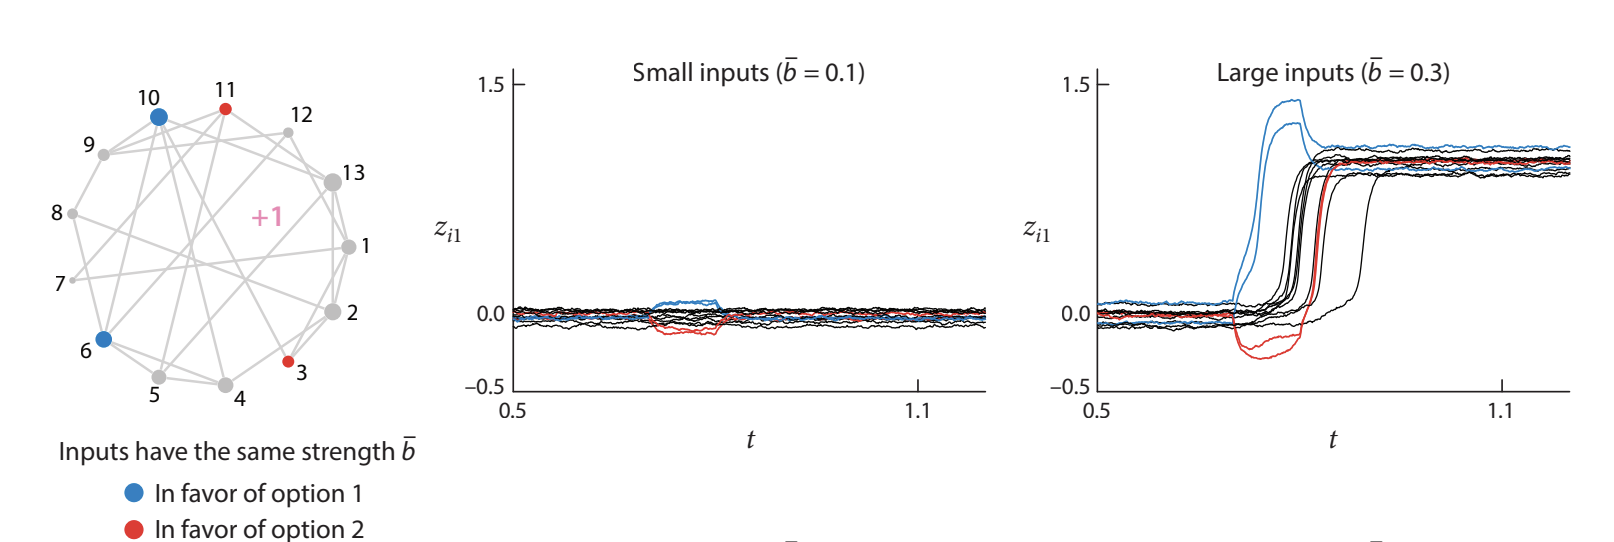
\includegraphics[width=\textwidth]{../plots/leonardfig2panA.png} 
		\caption{Results (Figure 2) of Leonard et al. 2024} \label{fig:damping1}
	\end{subfigure}
	
	\begin{subfigure}[t]{0.6\textwidth}
		\centering
		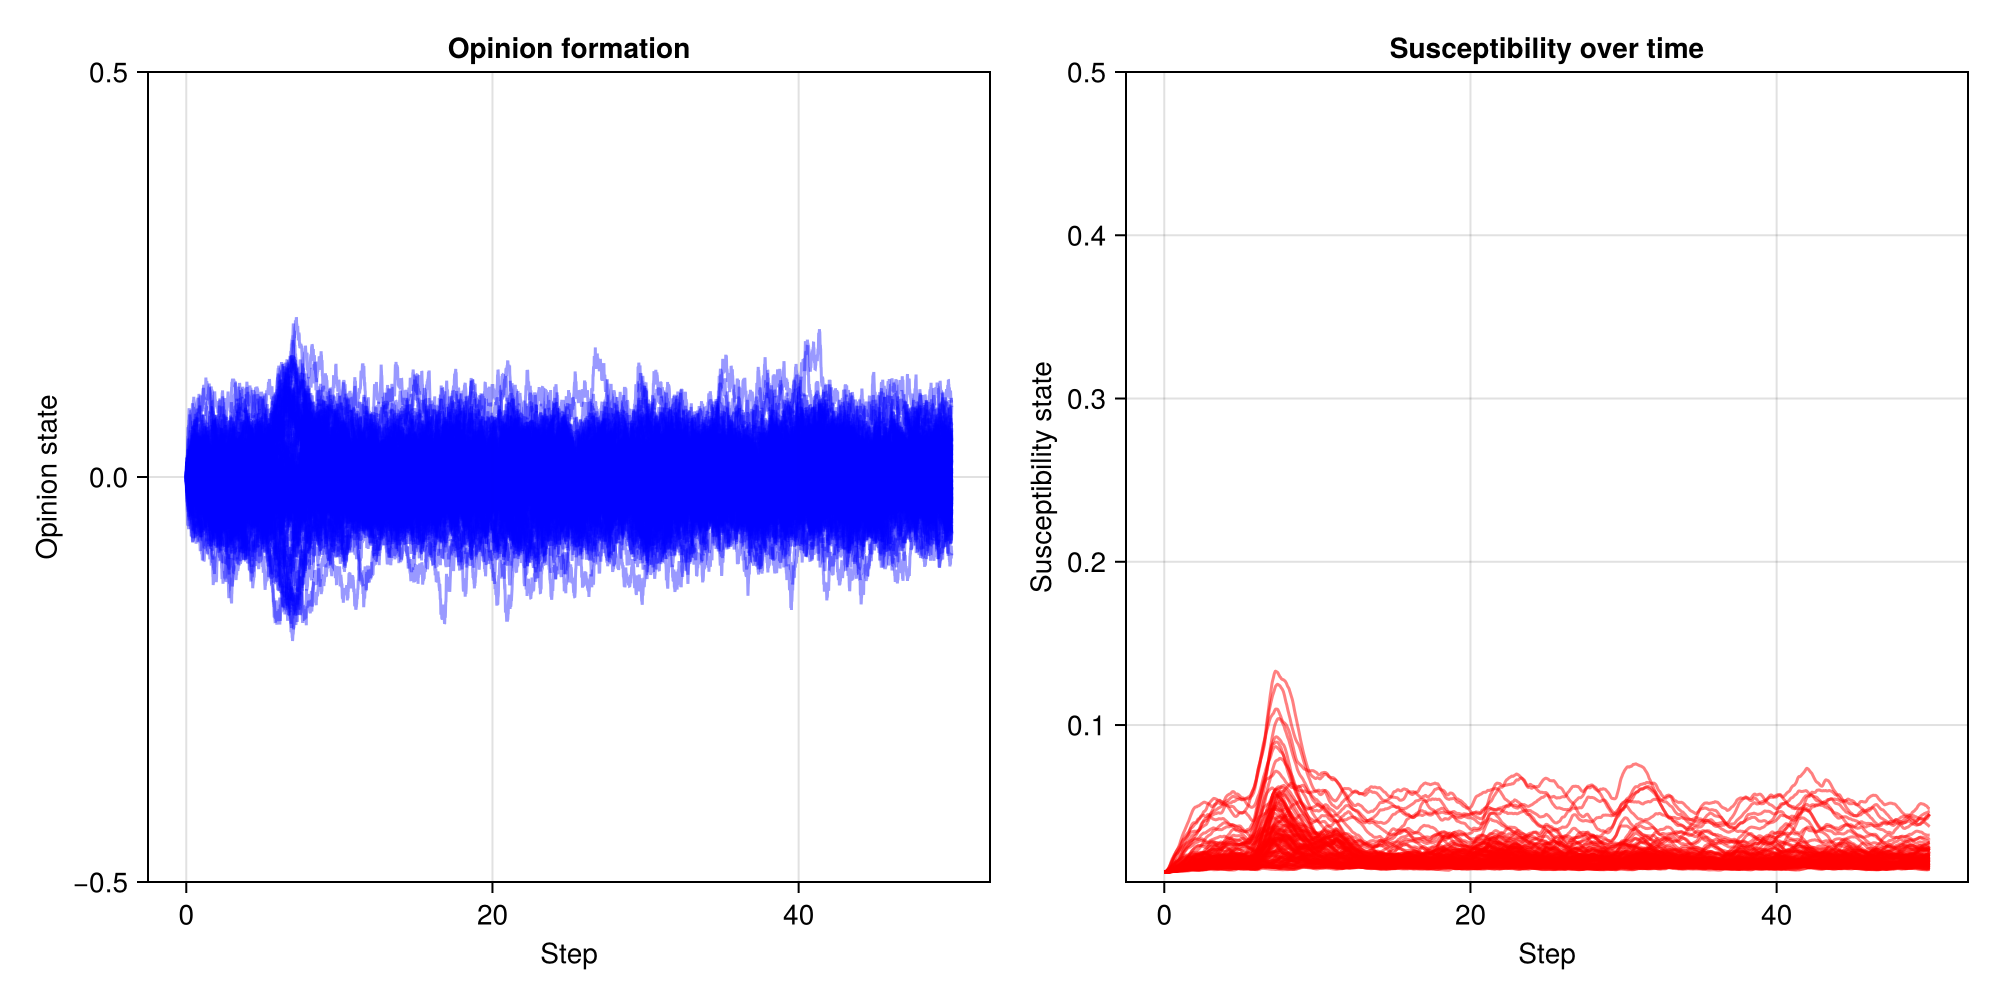
\includegraphics[width=\textwidth]{../plots/nog_constd_lowsig.png} 
		\caption{My simulation, input $b = \pm 0.1 $} \label{fig:damping2}
	\end{subfigure}
	
	\begin{subfigure}[t]{0.6\textwidth}
		\centering
		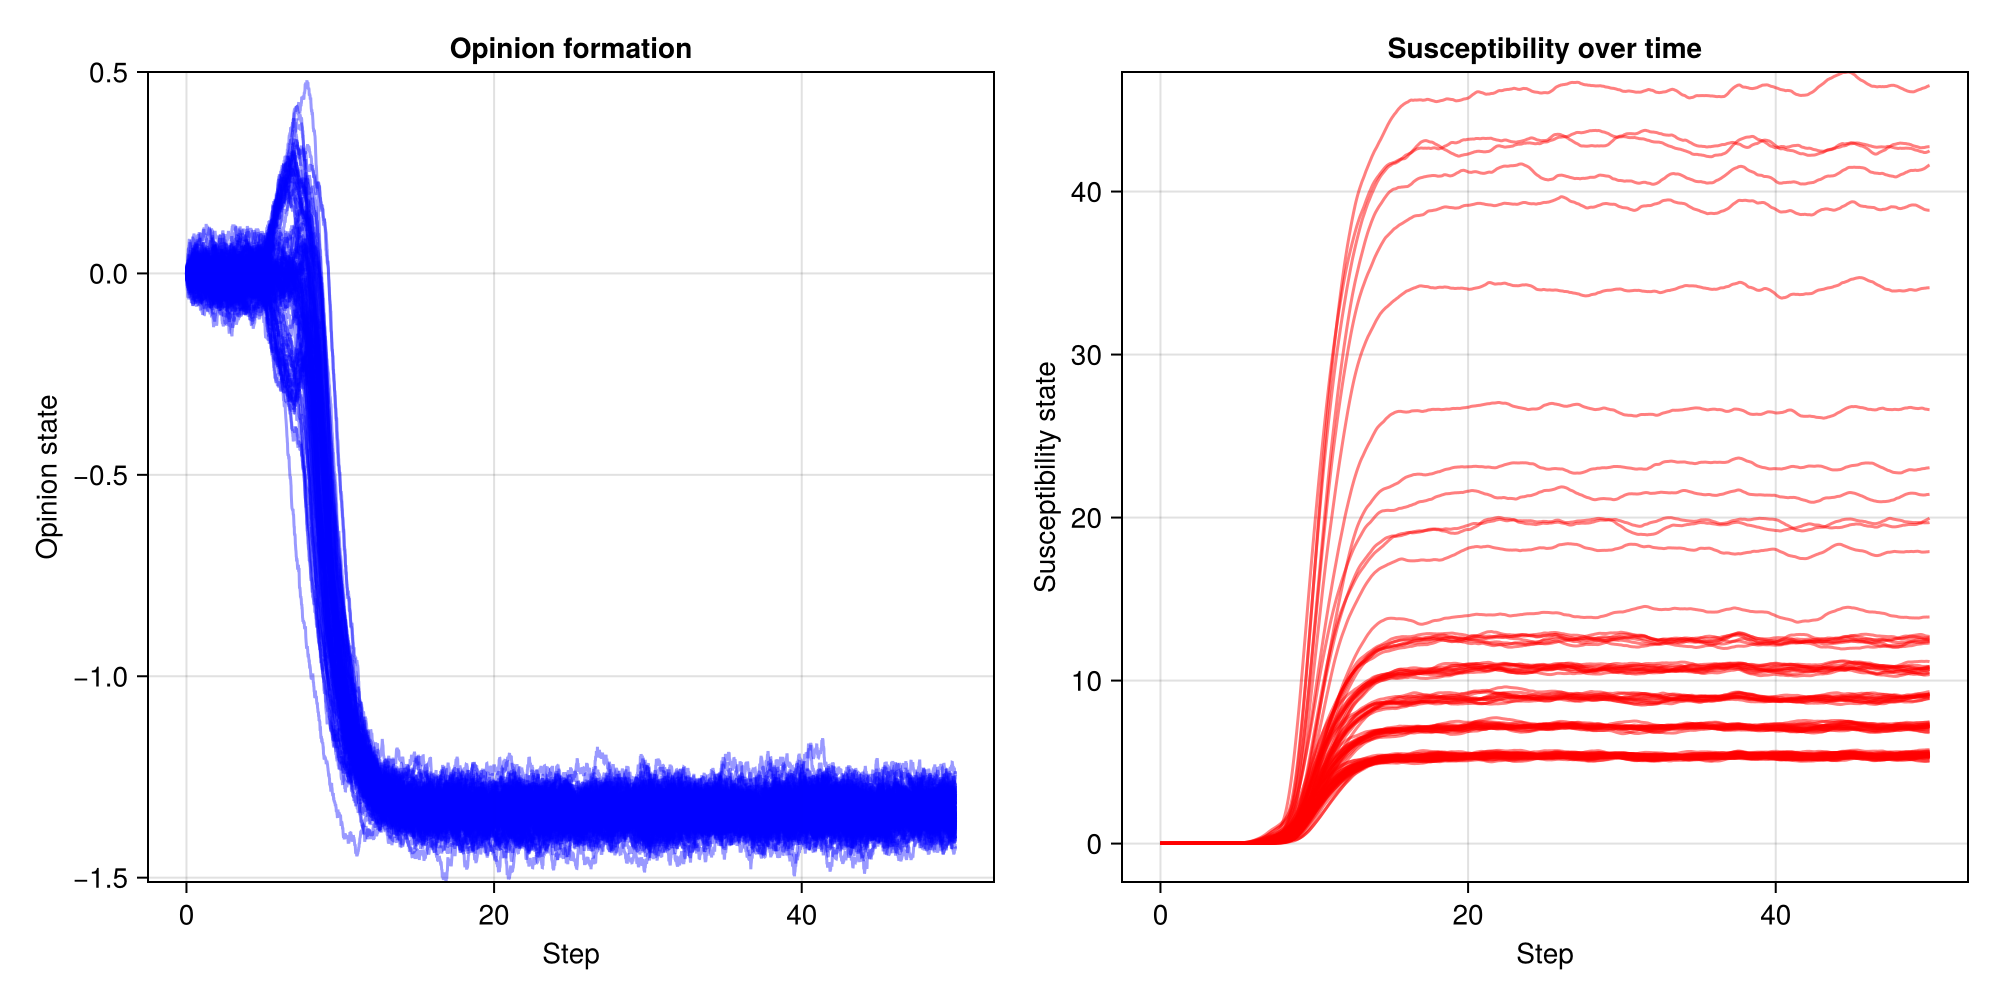
\includegraphics[width=\textwidth]{../plots/nog_constd_medsig.png} 
		\caption{My simulation, input $b = \pm 0.25 $} \label{fig:damping3}
	\end{subfigure}
	
	\caption{Opinion cascades under homogeneous damping, as external inputs grow larger. (\subref{fig:damping1}) is the top panel of Figure 2 of the BFL 2024 paper. In a small network of 13 agents, two agents receive a short signal of strength $b$ in favor of option 1 and concurrently, two agents receive a short signal of strength $-b$ in disfavor of option 1. Susceptibility state is not included. (\subref{fig:damping2}) and (\subref{fig:damping3}) are my simulations reproducing the same phenomena, with a network of 100 agents, with $d_i=d=0.75$. Opinion state in blue, susceptibility state in red. 25 agents receive a short signal in favor of option 1, while 25 other agents receive a similar signal in disfavor. }\label{fig:homdamping}
\end{figure}


\begin{figure}
	\centering
	\begin{subfigure}[t]{0.6\textwidth}
		\centering
		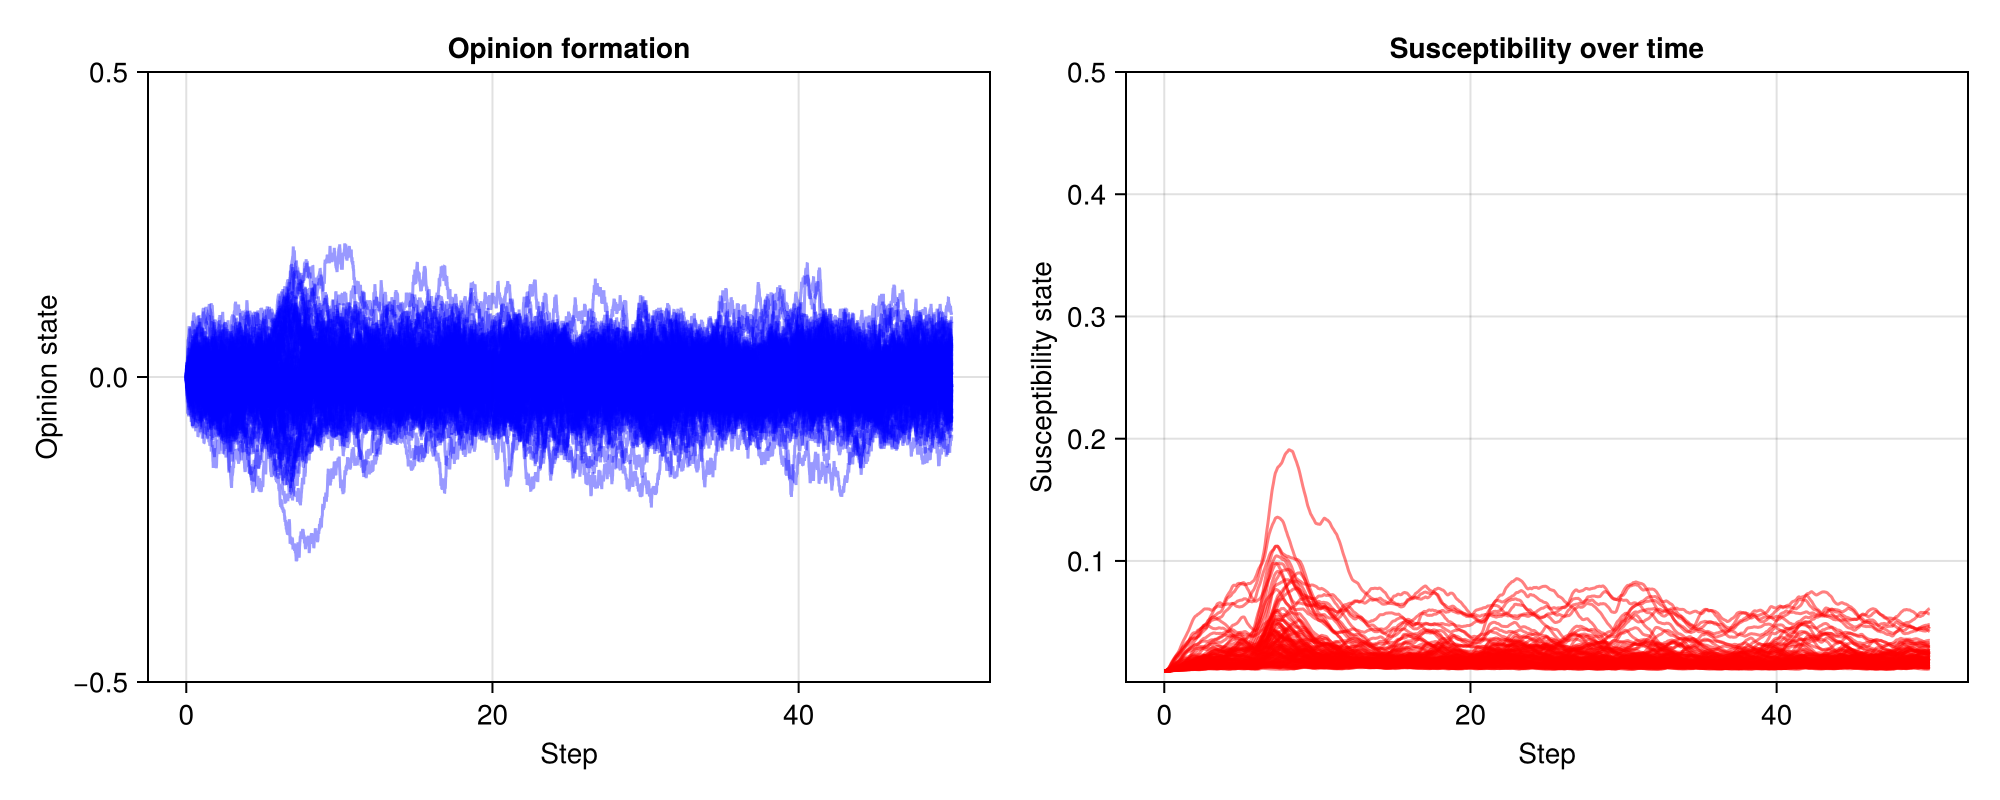
\includegraphics[width=\textwidth]{../plots/nog_hetd_lowsig.png} 
		\caption{My simulation, input $b = \pm 0.1 $} \label{fig:hetdamping1}
	\end{subfigure}
	
	\begin{subfigure}[t]{0.6\textwidth}
		\centering
		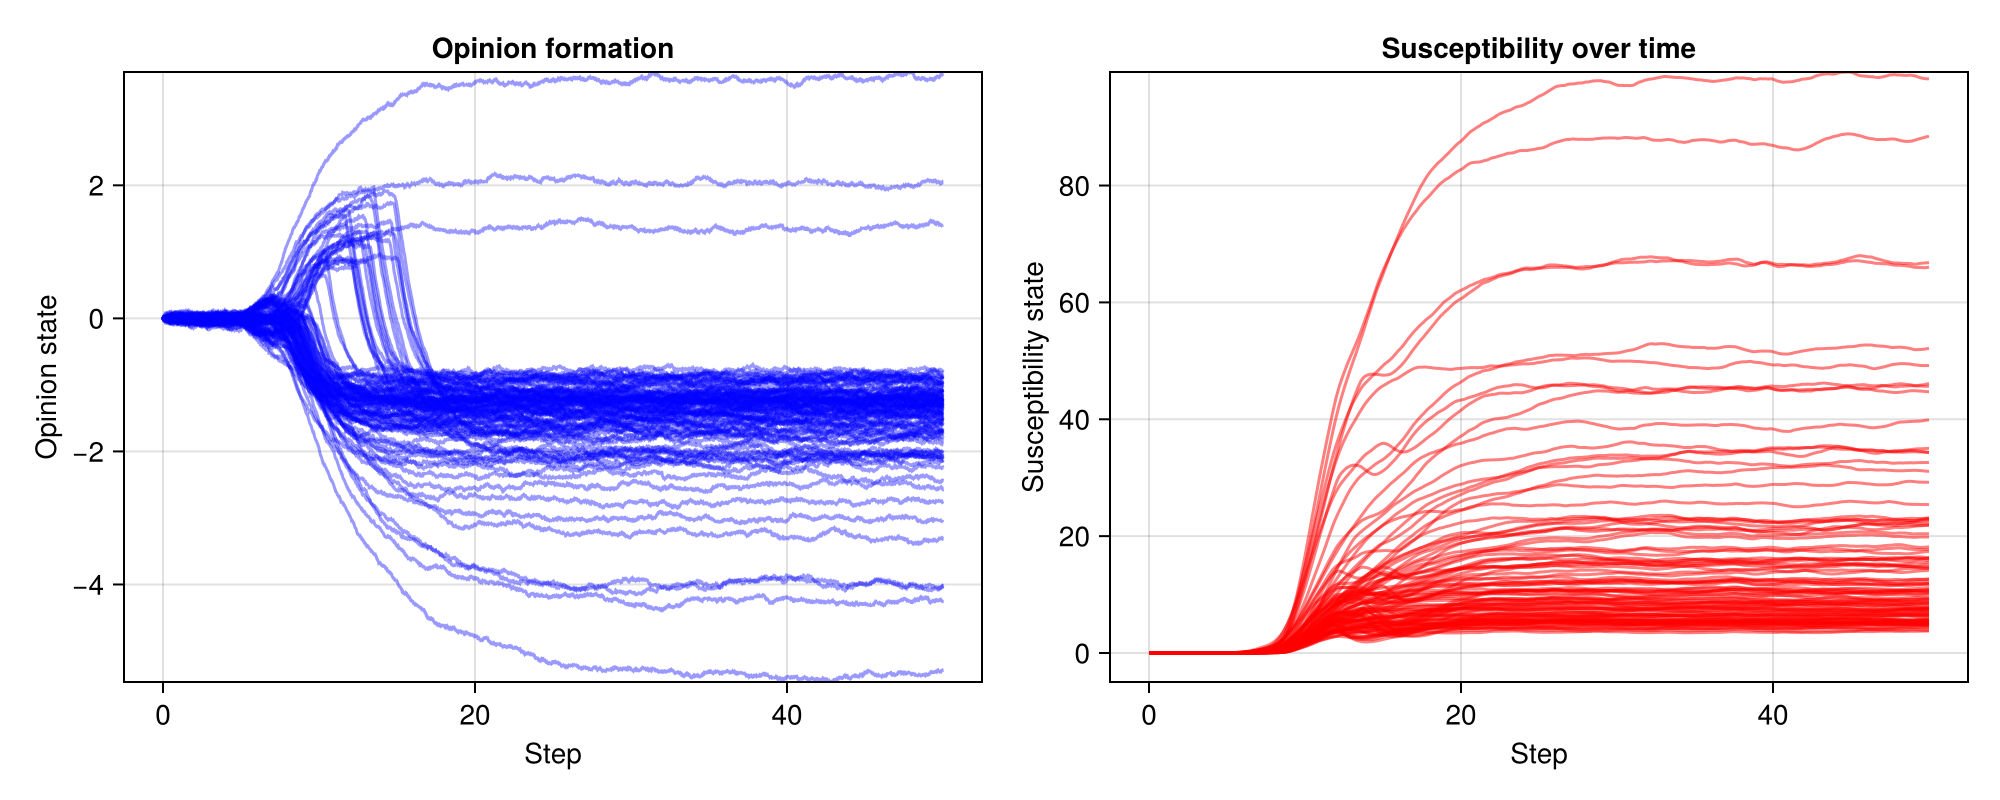
\includegraphics[width=\textwidth]{../plots/nog_hetd_medsig.png} 
		\caption{My simulation, input $b = \pm 0.25 $} \label{fig:hetdamping2}
	\end{subfigure}
	
	\caption{Opinion cascades under heterogeneous damping, as external inputs grow larger. My simulations, same conditions as Figure \ref{fig:homdamping} (b) and (c), but this time, $d_i \sim \mathcal{N}(0.75,0.25)$.}\label{fig:hetdamping}
\end{figure}

As can be seen in Figure \ref{fig:hetdamping}, a majority of agents converge to a similar opinion state, but a small number of agents converge to a more intense version of the majority view, while a smaller number still converge to the opposite view. This appears closer to real-life opinion dynamics, with a majority of agents getting moderately convinced, while some agents develop more extreme or contrarian views.

\subsection{Second modification: gating}

\begin{figure}
	\centering
	\begin{subfigure}[t]{0.6\textwidth}
		\centering
		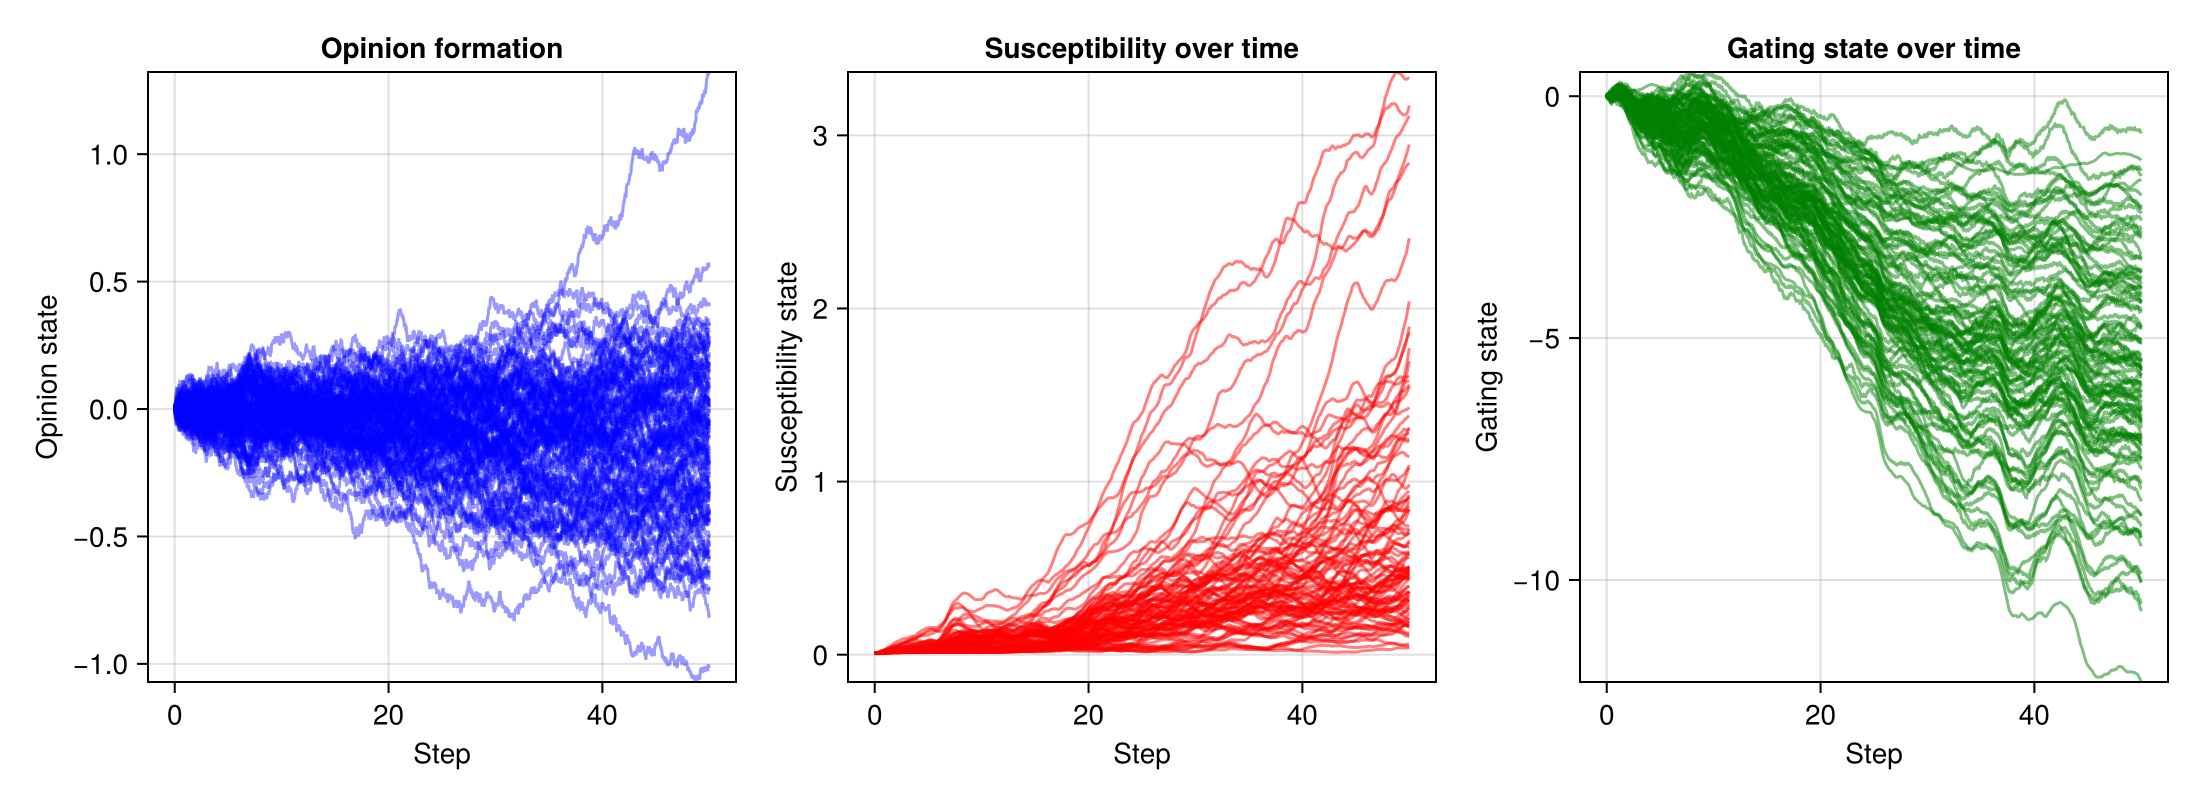
\includegraphics[width=\textwidth]{../plots/wg_hetd_lowsig.png} 
		\caption{My simulation, input $b = \pm 0.1 $} \label{fig:gating1}
	\end{subfigure}
	
	\begin{subfigure}[t]{0.6\textwidth}
		\centering
		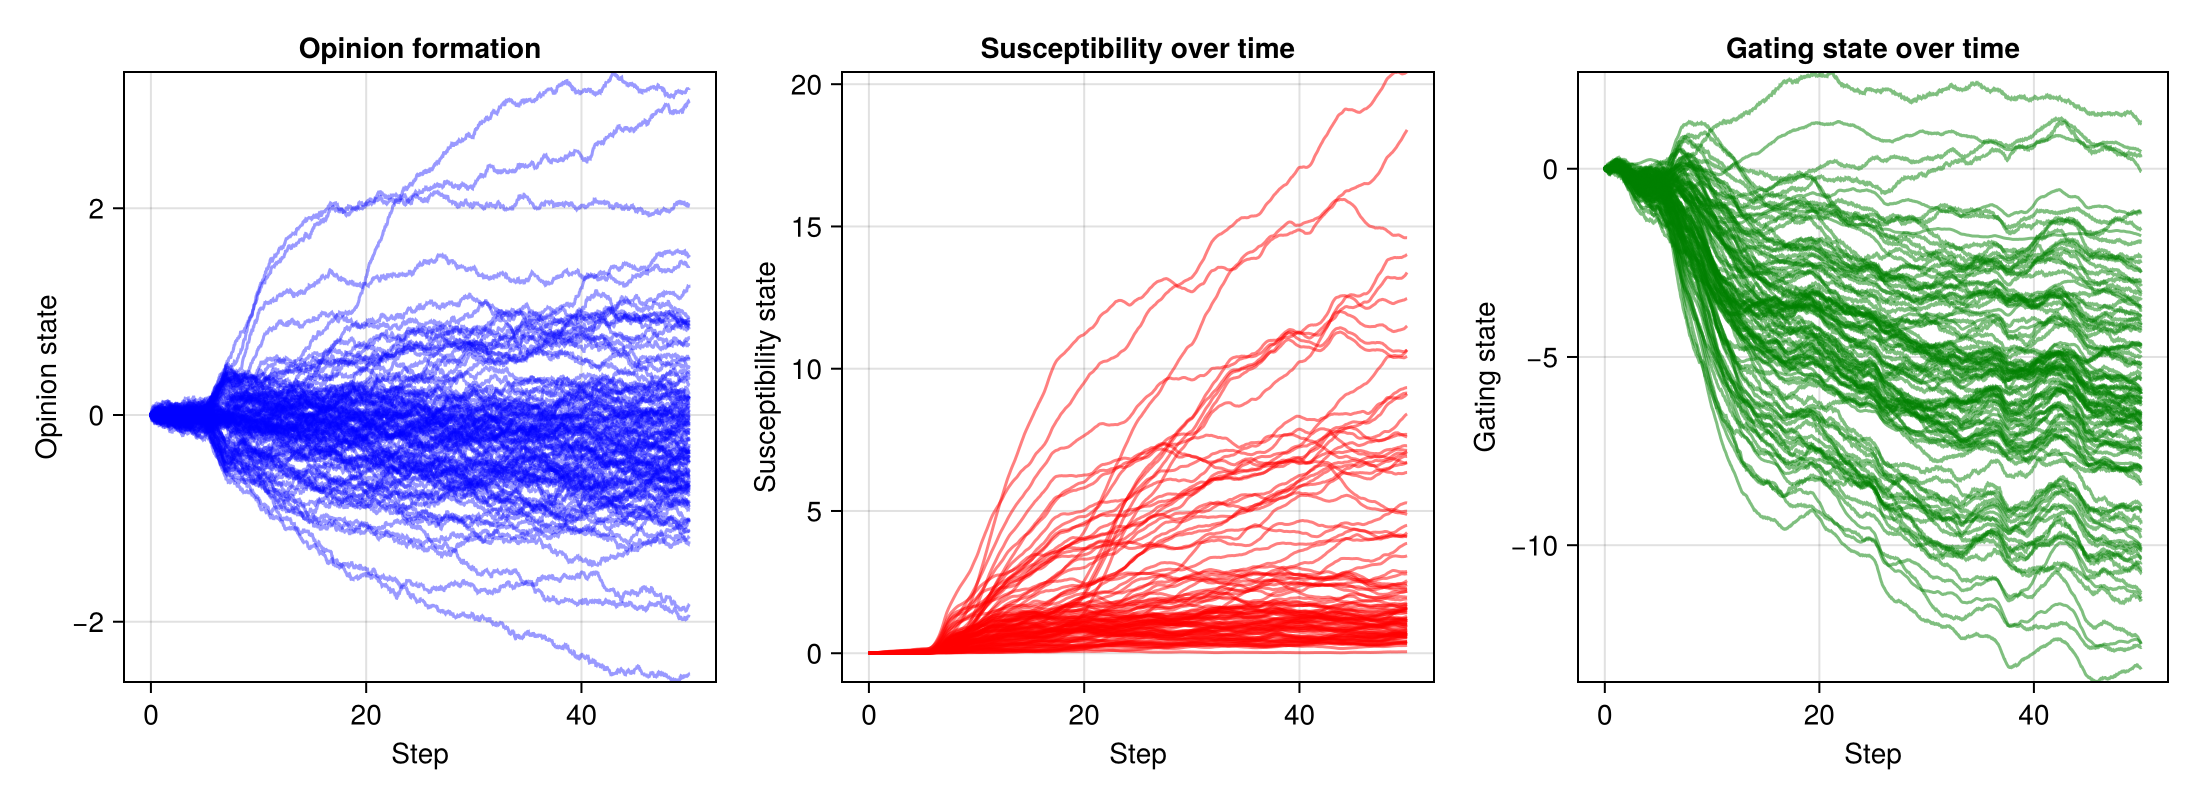
\includegraphics[width=\textwidth]{../plots/wg_hetd_medsig.png} 
		\caption{My simulation, input $b = \pm 0.25 $} \label{fig:gating2}
	\end{subfigure}
	
	\caption{Impact of naively adding an update gate to the model without further changes, with scaling factor $k_i \sim \mathcal{N}(1,0.5)$.}\label{fig:gatingintro}
\end{figure}

\section{Discussion}

\newpage

\section{Future directions}

\textbf{Building predictive models of the environment from partial information.} Building predictive models of their environment is a crucial component collective intelligence. Here, I take model building to mean the discovery of structure and regularity in a dynamic environment so that a system can predict its next inputs better than at random; such models can be implicit and behavioral (\cite{crutchfieldCalculiEmergenceComputation1994}). In real social networks, the information acquired by agents in order to do so is not only noisy, it is also partial and heterogeneous across agents. Settings of partial and heterogeneous information have rarely been explicitly studied in the network dynamics literature.

The BFL model only examines subjective beliefs, not the ability to converge to correct or useful answers. In the future, I plan to change the task from belief propagation to the collective recovery of a model of the environment from partial and heterogeneous information. A ground truth will exist, and I will examine under what conditions the network is successful at recovering it from noisy, partial and asymmetric inputs, including varying the distribution of information, noise, and other system parameters. This will be formalized in two ways, first as a static matrix reconstruction problem, and then as a dynamic hidden Markov problem.

Ongoing research efforts (\cite{malachAutoRegressiveNextTokenPredictors2023}) suggest that in some settings, next-token prediction of structured sequences may enable a model to learn complex data-generating processes (DGP) accurately. However, if and how a DGP can be recovered by a network when different nodes each receive noisy and imperfect measurements of the sequences remains unknown.

\textbf{Hysteresis as a mechanism for the reproduction of social inequality.} ...

\printbibliography[heading=bibintoc, title={References}]



\appendix

\section{Simulation results}

Contents

\end{document}